\documentclass{article}
\usepackage{listings}
\usepackage{ctex}
\usepackage{graphicx}
\usepackage[a4paper, body={18cm,22cm}]{geometry}
\usepackage{amsmath,amssymb,amstext,wasysym,enumerate,graphicx,caption,subfigure}
\usepackage{float,abstract,booktabs,indentfirst,amsmath}
\usepackage{array}
\usepackage{booktabs} %调整表格线与上下内容的间隔
\usepackage{multirow}
\usepackage{url}
\usepackage{diagbox}
\renewcommand\arraystretch{1.4}
\usepackage{indentfirst}
\setlength{\parindent}{2em}
\usepackage{listings}
\usepackage{xcolor}
\lstset{
	numbers=left, 
	numberstyle= \tiny, 
	keywordstyle= \color{ blue!70},
	commentstyle= \color{red!50!green!50!blue!50}, 
	frame=shadowbox, % 阴影效果
	rulesepcolor= \color{ red!20!green!20!blue!20} ,
	escapeinside=``, % 英文分号中可写入中文
	xleftmargin=2em,xrightmargin=2em, aboveskip=1em,
	basicstyle=\footnotesize,
	framexleftmargin=2em
} 


\geometry{left=2.8cm,right=2.2cm,top=2.5cm,bottom=2.5cm}
%\geometry{left=3.18cm,right=3.18cm,top=2.54cm,bottom=2.54cm}

\graphicspath{{figures/}}

\title{\heiti 数字电路实验报告 }

\begin{document}
	\vspace*{1cm}
	
	\begin{figure}[h]
		\centering
		
\includegraphics[scale=1.0]{xh.jpg}
	\end{figure}

	\vspace*{0.5cm}
	
	\begin{center}
		\Huge{\textbf{数字电路实验报告}}
	\end{center}
	
	\vspace{5cm}
	
	\begin{table}[h]
		\centering
		\begin{Large}
			\begin{tabular}{p{3cm} p{7cm}<{\centering}}
				实验题目: &  简单组合逻辑电路     \\ \cline{2-2}
				学生姓名:      & 孔浩宇   \\ \cline{2-2}
				学生学号: & PB20000113 \\ \cline{2-2}
				完成日期:       & 2022/10/20 \\ \cline{2-2}
			\end{tabular}
		\end{Large}		
	\end{table}
	\newpage
    \section{实验题目}
        \subsection*{\qquad 简单组合逻辑电路}

    \section{实验目的}
        \subsection*{\qquad (1)熟练掌握 Logisim 的基本用法}
        \subsection*{\qquad (2)进一步熟悉 Logisim 更多功能}
        \subsection*{\qquad (3)用 Logisim 设计组合逻辑电路并进行仿真}
        \subsection*{\qquad (4)初步学习 Verilog 语法}
    
    \section{实验环境}
        \subsection*{\qquad (1) PC 一台:Windows 操作系统/Java 运行环境(jre)}
        \subsection*{\qquad (2) Logisim 仿真工具 (vesion 2.7.1)}
    \clearpage
    \section{实验练习}
        \subsection*{1.用真值表自动生成电路}
        \begin{enumerate}
            \item [(a)]在Logisim中放入输入输出引脚 (图1.1)
            \begin{figure*}[htbp]
                \centering
                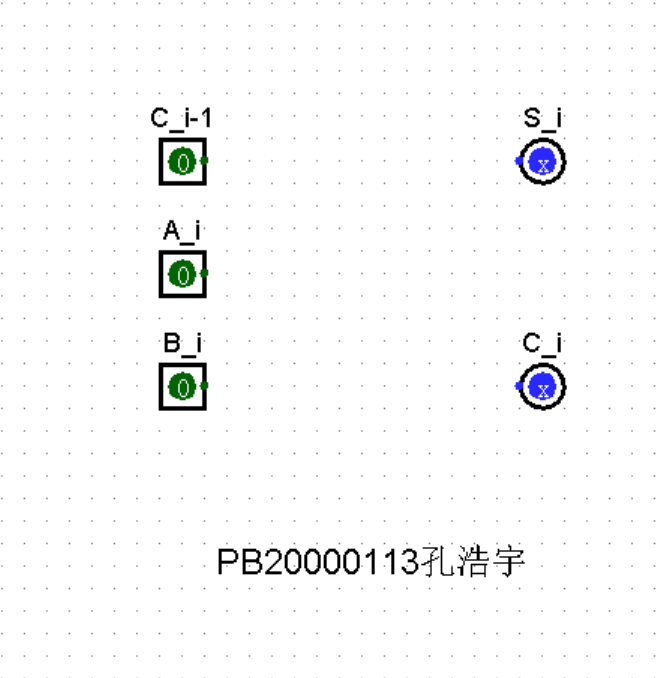
\includegraphics[scale=0.5]{t11.png}
                \caption*{图1.1}
            \end{figure*}
            \item [(b)]在菜单栏的$'Project'$选项卡中找到$'Analyze Circuit'$选项,
            选择$'Table'$选项,按照真值表修改输出值,并生成电路 (图1.2)
            \begin{figure*}[htbp]
                \centering
                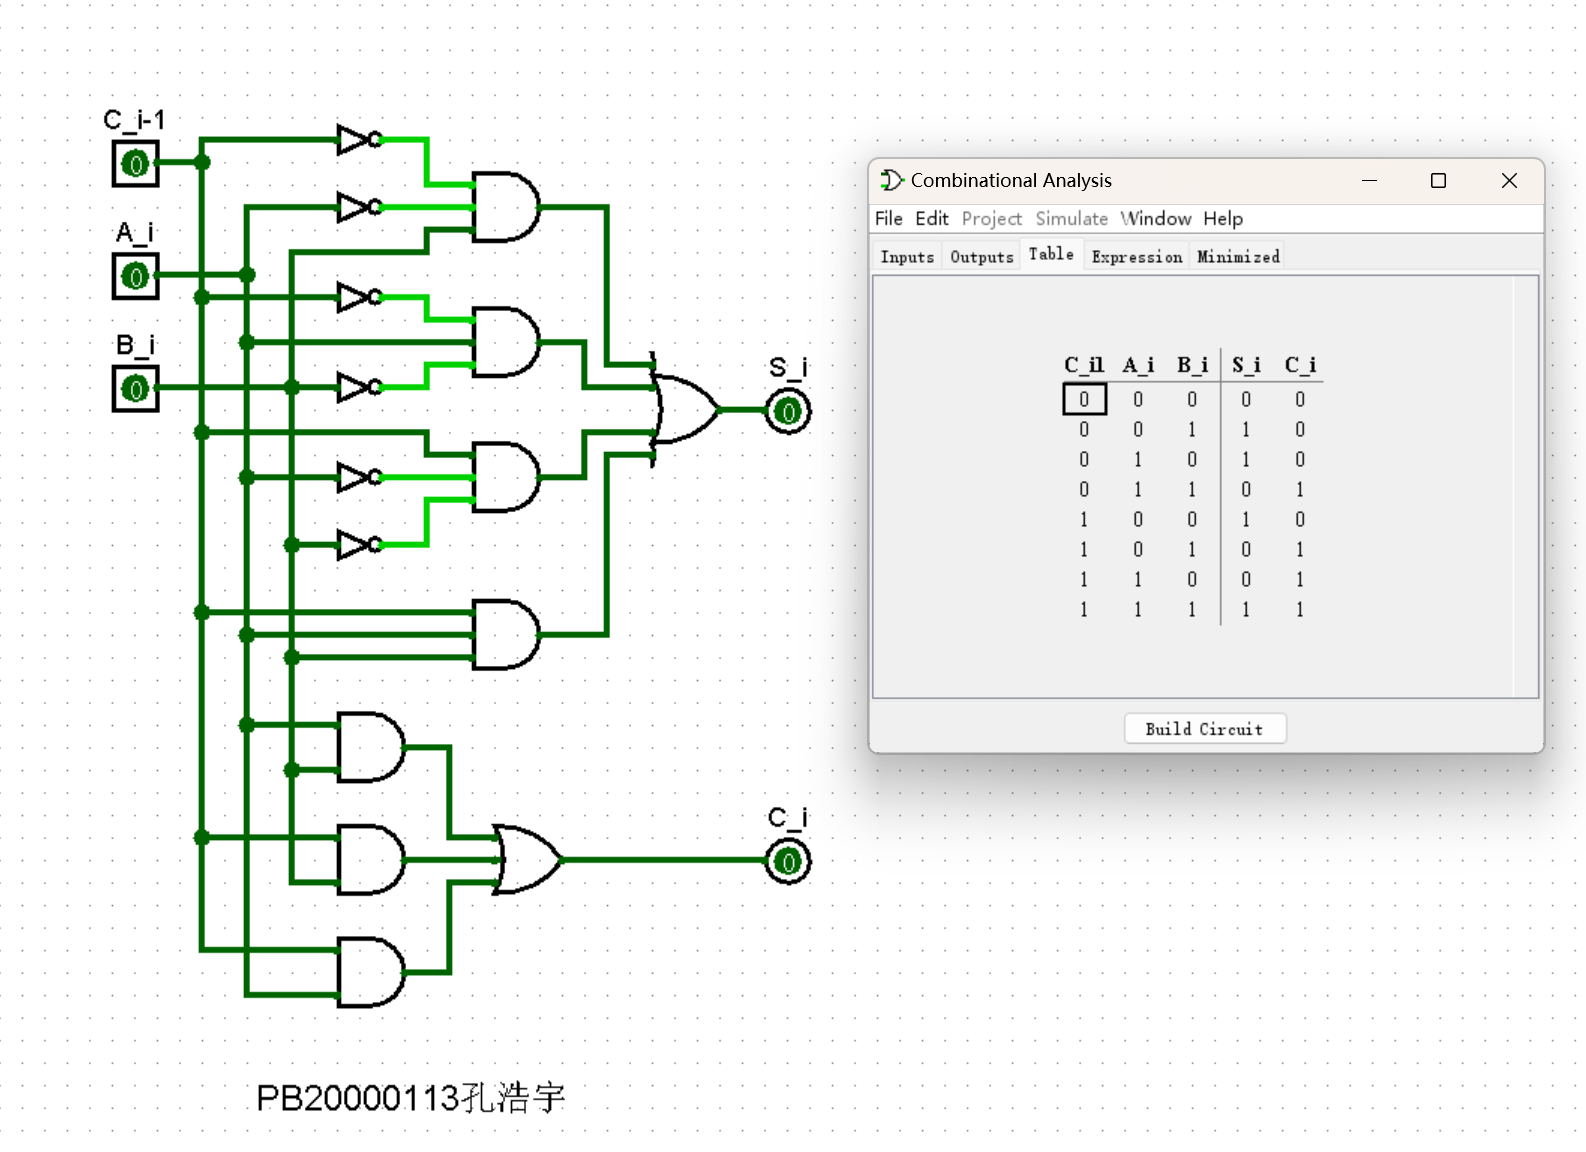
\includegraphics[scale=0.5]{t12.png}
                \caption*{图1.2}
            \end{figure*}
        \end{enumerate}
        \clearpage
        \subsection*{2.用表达式自动生成电路}
        \begin{enumerate}
            \item [(a)]根据真值表写出各输出信号的表达式并借助$'Minimized'$进行化简 (图2.1)
            \begin{figure*}[htbp]
                \centering
                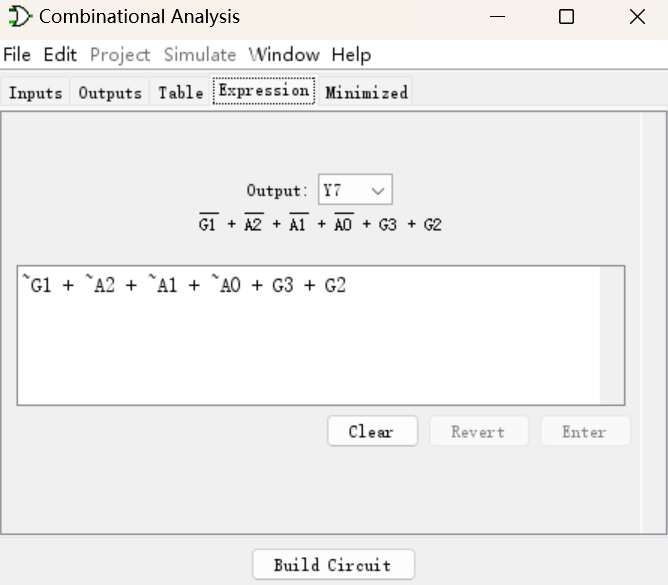
\includegraphics[scale=0.5]{t21.png}
                \caption*{图2.1}
            \end{figure*}
            \item [(b)]生成电路 (图2.2)
            \begin{figure*}[h]
                \centering
                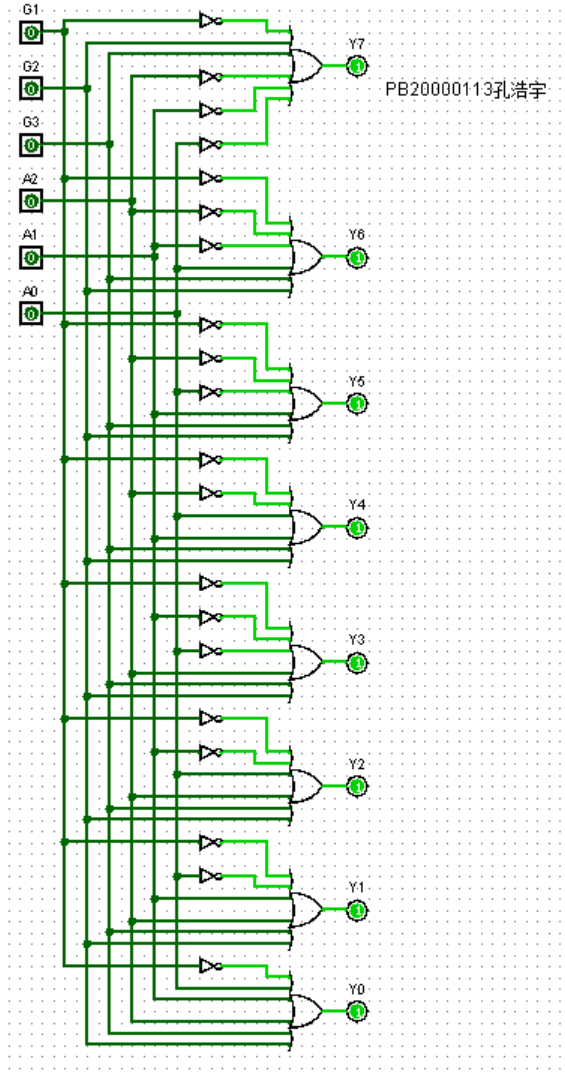
\includegraphics[scale=0.6]{t22.png}
                \caption*{图2.2}
            \end{figure*}
        \end{enumerate}
        \clearpage
        \subsection*{3.二选一数据选择器}
        \begin{enumerate}
            \item [(a)]电路图如图 (图3.1)
            \begin{figure*}[htbp]
                \centering
                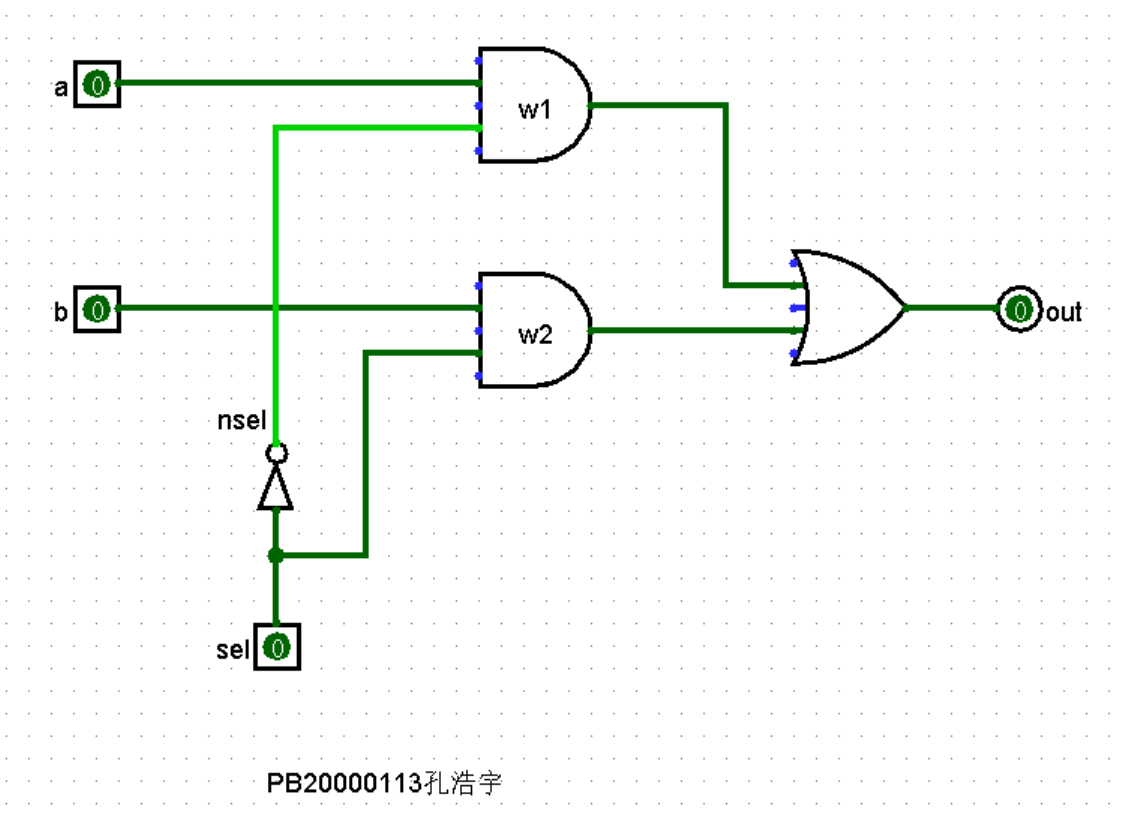
\includegraphics[scale=0.45]{t31.png}
                \caption*{图3.1}
            \end{figure*}
            \item [(b)]Verilog代码如下 (图3.2)
            \begin{figure*}[htbp]
                \centering
                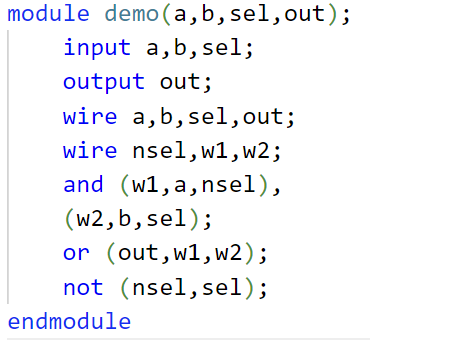
\includegraphics[scale=0.8]{t3v.png}
                \caption*{图3.2}
            \end{figure*}
        \end{enumerate}
        \clearpage
        \subsection*{4.四选一数据选择器}
            \begin{enumerate}
                \item [(a)]将二选一选择器电路进行封装 (图4.1)
                \begin{figure*}[htbp]
                    \centering
                    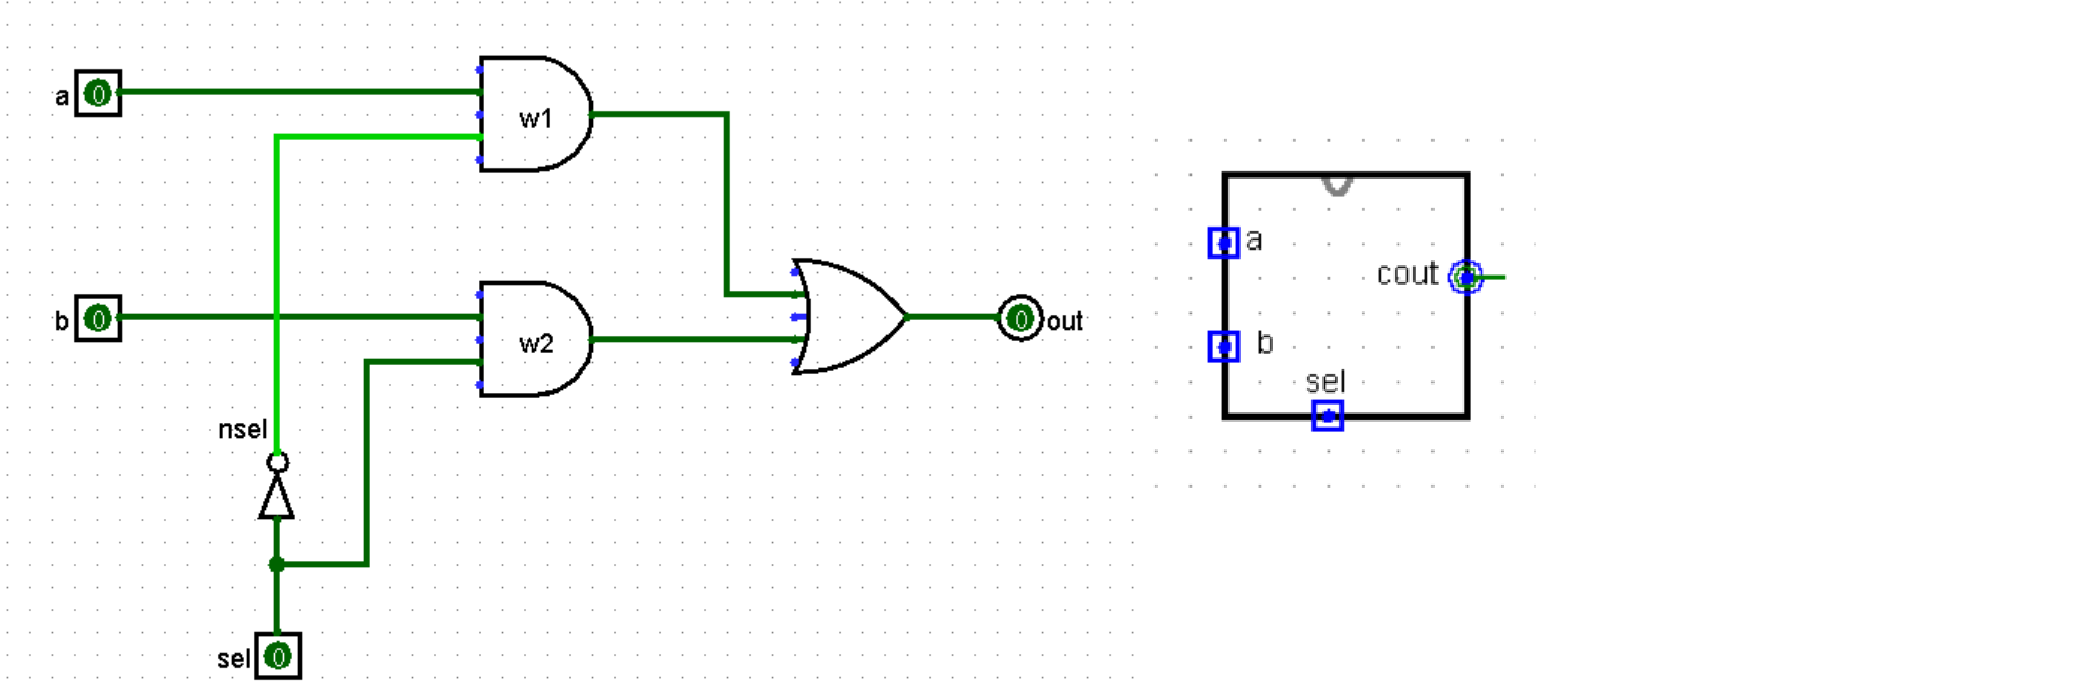
\includegraphics[scale=0.5]{t41.png}
                    \caption*{图4.1}
                \end{figure*}
                \item [(b)]绘制四选一数据选择器 (图4.2)
                \begin{figure*}[htbp]
                    \centering
                    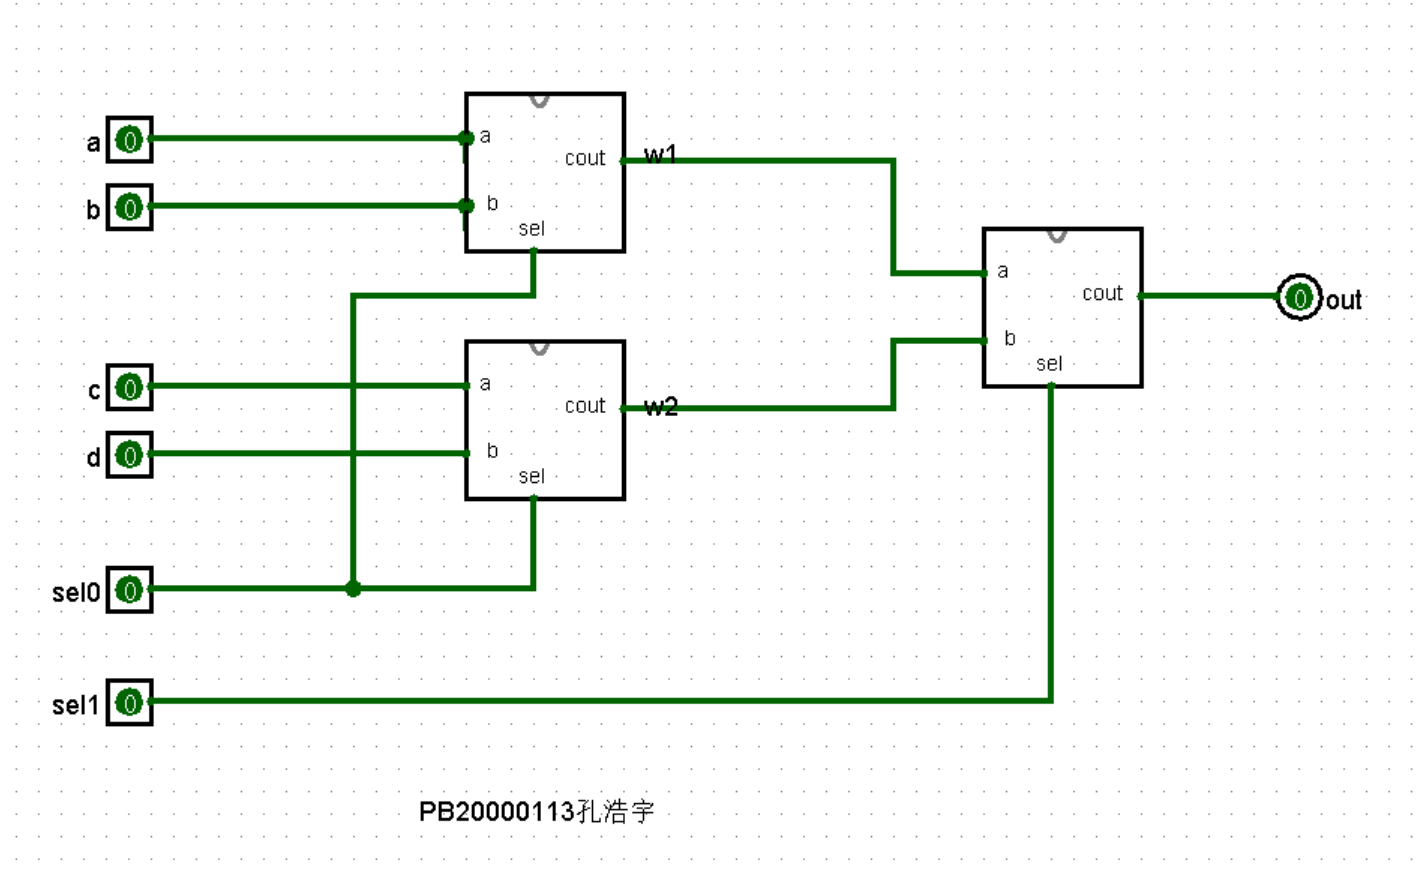
\includegraphics[scale=0.6]{t42.png}
                    \caption*{图4.2}
                \end{figure*}
                \item [(c)]编写Verilog代码 (图4.3)
                \begin{figure*}[htbp]
                    \centering
                    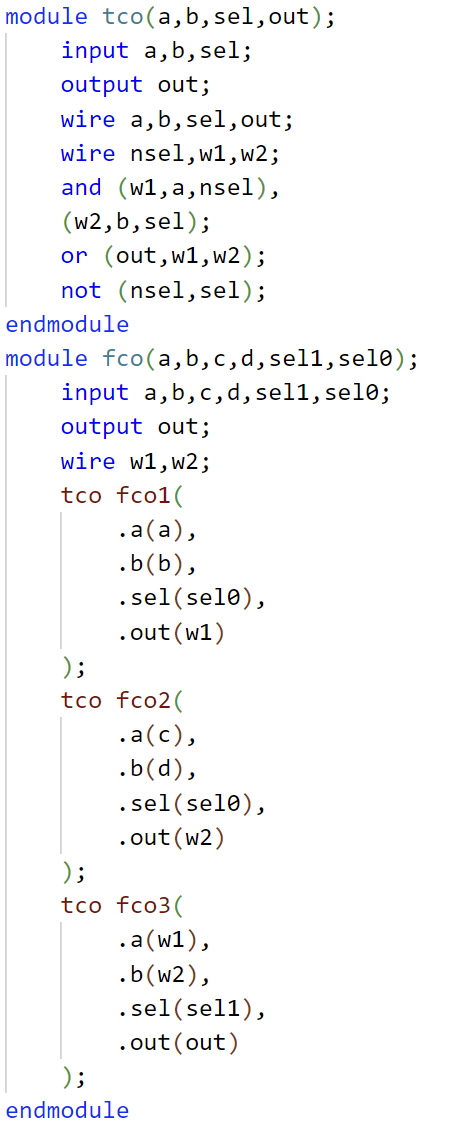
\includegraphics[scale=1]{t4v.png}
                    \caption*{图4.3}
                \end{figure*}
            \end{enumerate}
        \clearpage
        \subsection*{5.八位优先编码器Verilog代码}
            \begin{enumerate}
                \item []Verilog代码如下 (图5.1)
                \begin{figure*}[htbp]
                    \centering
                    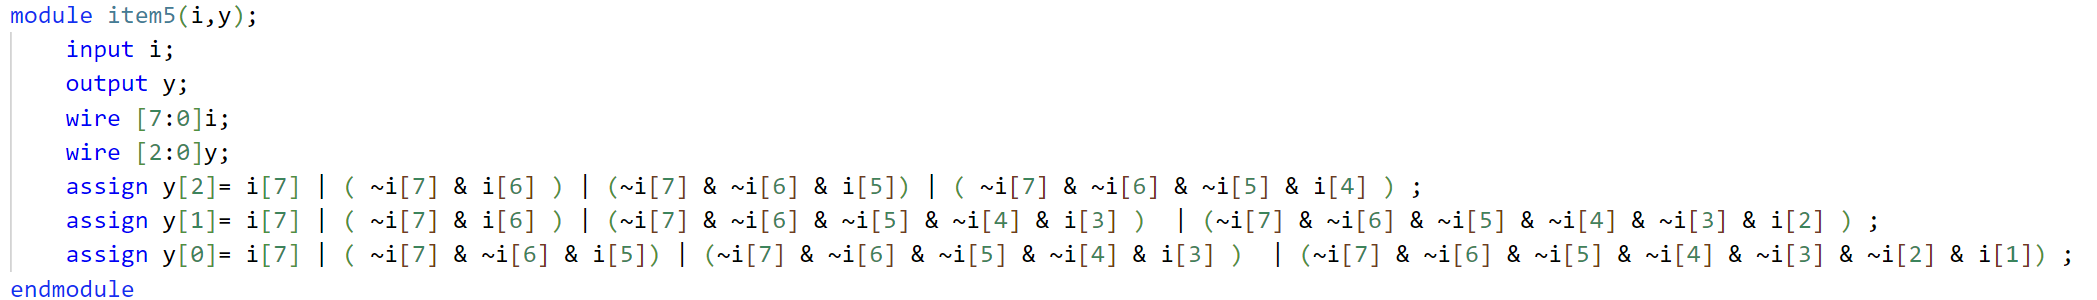
\includegraphics[scale=0.5]{t5v.png}
                    \caption*{图5.1}
                \end{figure*}
            \end{enumerate}

        \subsection*{6.阅读verilog代码画电路}
            \begin{enumerate}
                \item [(a)]绘制电路图如下 (图6.1)
                \begin{figure*}[htbp]
                    \centering
                    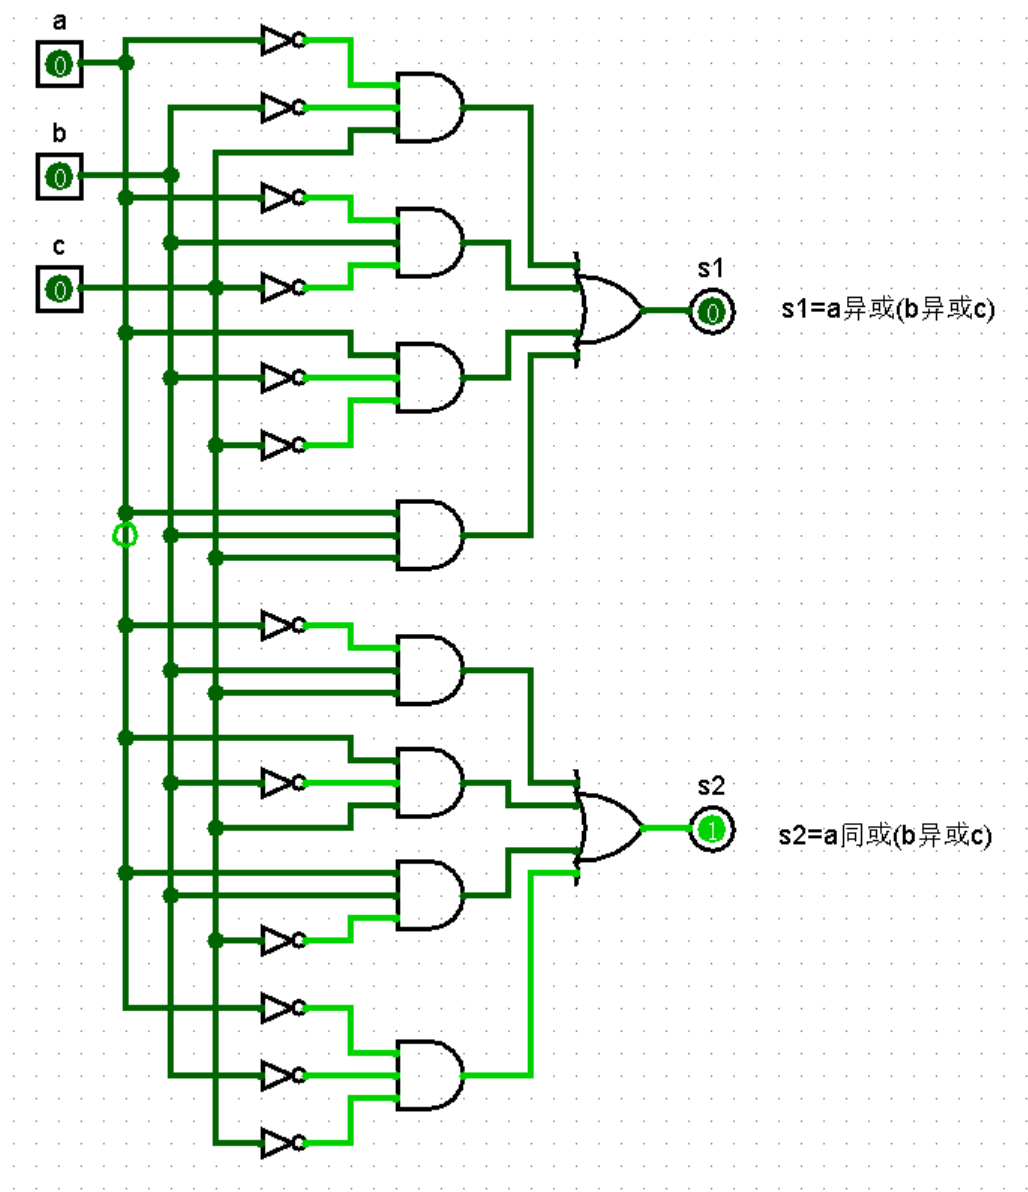
\includegraphics[scale=0.5]{t61.png}
                    \caption*{图6.1}
                \end{figure*}
                \item [(b)]当abc中1的个数为奇数时,s1为1,s2为0;1的个数为偶数时,s2为1,s1为0.
            \end{enumerate}
    \clearpage
    \section{总结与思考}
	\begin{enumerate}
        \item [-]学会了使用真值表和表达式生产电路
        \item [-]初步学习了Verilog语法
        \item [-]本次实验难易程度适中,任务量适中
        \item [-]对Verilog代码编写不熟练,暂不知道如何判断正误
    \end{enumerate}
\end{document}